\par
Nous avons choisi au début du projet d'utiliser une structure XML pour représenter les données stockées dans le QR Code (voir \ref{representationDonnees}). Ce choix était motivé principalement par la facilité de gestion du XML en Javascript.
\par
Le XML a toutefois posé des problèmes au niveau de la concision des QR Codes générés. Nous avons tenté de remplacer la structure XML par une structure JSON plus concise lors de la première semaine de décembre, mais nous avions déjà trop de dépendances au XML. Nous avons alors tenté d'utiliser des librairies convertissant le XML déjà généré en JSON avant l'insertion des données dans le QR Code, mais nous n'en avons trouvé aucune suffisamment fiable (les attributs des noeuds XML étaient très mal gérés, et les noeuds de même nom étaient fusionnés sans respecter leur ordre).\\
\par
Nous nous sommes donc orientés vers une solution de compression pour compenser l'intérêt qu'avait le JSON sur le XML. La solution que nous avons adoptée consiste à remplacer toutes les chaînes de caractères connues constituant le XML par un caractère UTF-8\footnote{UTF-8 (abréviation de l’anglais Universal Character Set Transformation Format - 8 bits) est un codage de caractères informatiques conçu pour coder l’ensemble des caractères du « répertoire universel de caractères codés » (Wikipédia)} prédéfini. Notre choix s'est porté sur les caractères de l'alphabet cyrillique car la probabilité qu'ils soient utilisés par les utilisateurs de l'application est très faible, et ils ne sont codés que sur deux octets (les caractères de l'UTF-8 sont représentés sur un nombre d'octets variant de un à quatre). Nous avons donc fait l'inventaire de toutes les chaînes de caractères de longueur supérieure à deux apparaissant dans notre représentation XML, et nous avons attribué à chacune un caractère de l'alphabet cyrillique. La classe \classe{CompresseurTexte} du Contrôleur se charge de remplacer par le caractère correspondant toutes les chaînes de caractères appartenant à la représentation d'un QR Code avant qu'il ne soit généré.\\
\par
Nous avons rendu cette solution la plus évolutive possible, en ajoutant deux caractères prédéfinis au début de la chaîne compressée pour notifier qu'elle a été compressée, et donc laisser la possibilité à l'application mobile avec un test simple d'interpréter les QR Codes n'ayant pas subi la compression. Le premier caractère inséré est le premier caractère de l'alphabet cyrillique, et le second est le chiffre 1, indiquant qu'il s'agit de la première version de cette méthode de compression. D'autres versions de la compression pourront ainsi être proposées dans le futur si la structure XML de représentation des données est modifiée.\\
\par
Le principal inconvénient de cette solution est qu'elle ne compresse que la représentation des données et pas les données elles-mêmes. Un QR Code contenant beaucoup de texte sera toujours volumineux. Elle est toutefois très efficace pour les QR Codes contenant peu de données comme en témoigne l'exemple ci-dessous.

\begin{figure}[!h]
\begin{adjustbox}{minipage=\textwidth,bgcolor={RGB}{240 240 240}}

\lstset{language=XML}

\begin{lstlisting}
<donneesutilisateur xmlns="http://www.w3.org/1999/xhtml" type="atomique">
  <contenu>
    <texte>Le lion appartient a la famille des felides</texte>
  </contenu>
  <famille nom="animaux" ordre="3"></famille>
</donneesutilisateur>

\end{lstlisting}

\end{adjustbox}
\caption{Données stockées dans un QR Code simple sans compression (214 octets)}

\end{figure}\textbf{}


\begin{figure}[!h]
	\centering
   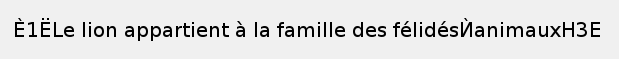
\includegraphics[scale=0.4]{img/compression.png}
   \caption{Données stockées dans un QR Code simple avec compression (63 octets, soit un gain de 70\%)}
\end{figure}